\chapter{Beschreibung des 5G-AKA Protokolls}
\label{chap:2}

Das 5G-AKA-Protokoll ist eines von mehreren Protokollen des 5G-Standards.
Vor Allem das EAP-AKA-Protokoll und das 5G-AKA-Protokoll sind für den sicheren Austausch eines kryptographischen Schlüssels zuständig. 
Bei beiden Protokollen ist der erste Teil identisch, bis bei dem Provider eines der Protokolle ausgewählt wird. %3GPP TS 33.501 V15.34.1 Page 40
Bei beiden Protokollen ist auch der Authentifizierungsvorgang sehr ähnlich, wobei das 5G-AKA-Protokoll gegenüber dem EAP-AKA-Protokoll dahingehen erweitert wurde, dass es dem Provider, \textit{Home Network} genannt, eine erfolgreiche Authentifizierung nachweist. %3GPP TS 33.501 V15.34.1 Page 43

Das 5G-AKA-Protokoll wird größtenteils in der Spezifikation TS 33.501 des 3GPP beschrieben. %3GPP TS 33.501 V15.34.1
Dabei wird immer die zum Zeitpunkt dieser Arbeit neueste Version V15.34.1 herangezogen.

\section{Ziele}

Ziel des 5G-AKA Protokolls ist es den Benutzer und das Netzwerk gegenseitig zu authentifizieren (\textit{Mutual Authentication}) und Schlüsselmaterial bereitzustellen, die von nachfolgenden Protokollen verwendet werden können. % 3GPP TS 33.501 V15.34.1 Page 37
Bei einer erfolgreichen Authentifizierung wissen alle Teilnehmer des Protokolls über den Erfolg Bescheid und es wurde ein gemeinsamer \textit{Anchor Key} ausgetauscht.
Aus diesem \textit{Anchor Key} können weitere Schlüssel für mehrere Sicherheitskontexte abgeleitet werden.
Ein Überblick über die ableitbaren Schlüssel ist in Abbildung 6.2.1-1 und 6.2.2-1 des 3GPP TS 33.501 V15.34.1 zu finden. % 3GPP TS 33.501 V15.34.1 Page 49 & 52

\section{Das Protokoll}

\subsection{Entitäten}% Auf die Sicherheitsstandards für die Kommunikation zwischen den Entitäten eingehen.

In dem Protokoll werden vier grundlegende Entitäten beschrieben.
Diese sind das \gls{ue}, die \gls{seaf}, die \gls{ausf} und das \gls{udm}.

\glsreset{ue}
\subsubsection{\gls{ue}}

Das \gls{ue} kann sich zum Beispiel auf dem Smartphone des Nutzers oder auf einem 5G-USB Dongle befinden.
Es lässt sich in das \gls{me} und das \gls{usim} unterteilen.
In dem \gls{usim} werden für die Authentifizierung benötigte Schlüssel und Benutzerkennungen gespeichert, die für die eindeutige Identifizierung und Authentifizierung des \gls{ue} benötigt werden. %3GPP TS 33.501 V15.34.1 Page 24
In dem \gls{me} werden die Schlüssel, die für die Kommunikation nach dem 5G-AKA-Protokoll benötigt werden, berechnet.

\glsreset{seaf}
\subsubsection{\gls{seaf}}

Die \gls{seaf} ist Teil des mit dem \gls{ue} kommunizierenden Netzwerks, auch \textit{Serving Network} genannt.
Sie kommuniziert mit dem \gls{ue} und mit dem Provider des Benutzers.
Nach erfolgreicher Authentifizierung haben das \gls{ue} und die \gls{seaf} beide einen gemeinsamen Schlüssel.%3GPP TS 33.501 V15.34.1 Page 37

\glsreset{ausf}
\subsubsection{\gls{ausf}}

Die \gls{ausf} ist Teil des Providers, bei dem sich der Benutzer die hier verwendete SIM-Karte gekauft hat, auch \textit{Home Network} genannt.
Sie kommuniziert mit der \gls{seaf} und validiert die Antwort des \gls{ue} für die \gls{seaf}.

\glsreset{udm}
\subsubsection{\gls{udm}}

Das \gls{udm} ist, wie auch die \gls{ausf} Teil des \textit{Home Network}.
Grundsätzlich funktioniert es jedoch nicht ohne die \gls{arpf} und die \gls{sidf}.

Das \gls{udm} und die \gls{arpf} generieren Authentifizierungsvektoren aus den Schlüsseln, die sie mit dem \gls{usim} teilen.
Die \gls{sidf} berechnet die Benutzerkennung (\glsunset{supi}\gls{supi}) für das \gls{udm} und die \gls{arpf} aus einer verschlüsselten Benutzerkennung (\glsunset{suci}\gls{suci}), die sie von dem \gls{ausf} erhält.


\subsection{Vorbedingungen}

Damit das 5G-AKA Protokoll erfolgreich durchgeführt werden kann müssen folgende Vorbedingungen erfüllt sein:

\begin{itemize}
\item Das \gls{usim} und das \gls{udm}/\gls{arpf} verfügen über den gemeinsamen Langzeitschlüssel \gls{k}.

\item Die \gls{arpf} verfügt über den privaten Schlüssel und das \gls{usim} verfügt über den öffentlichen Schlüssel eines asynchronen Schlüsselpaars.

\end{itemize}


\subsection{Authentifikationsprozedur}

Die \cref{fig:protocol_v1} zeigt eine erfolgreiche Authentifizierung.
Nach dem Ende der Prozedur haben sich alle Entitäten auf den \textit{Anchor Key}, \gls{k-seaf}, geeinigt.
Dieser wird als Grundlage für die weitere Kommunikation verwendet.

\begin{figure}[H]
  \centering
  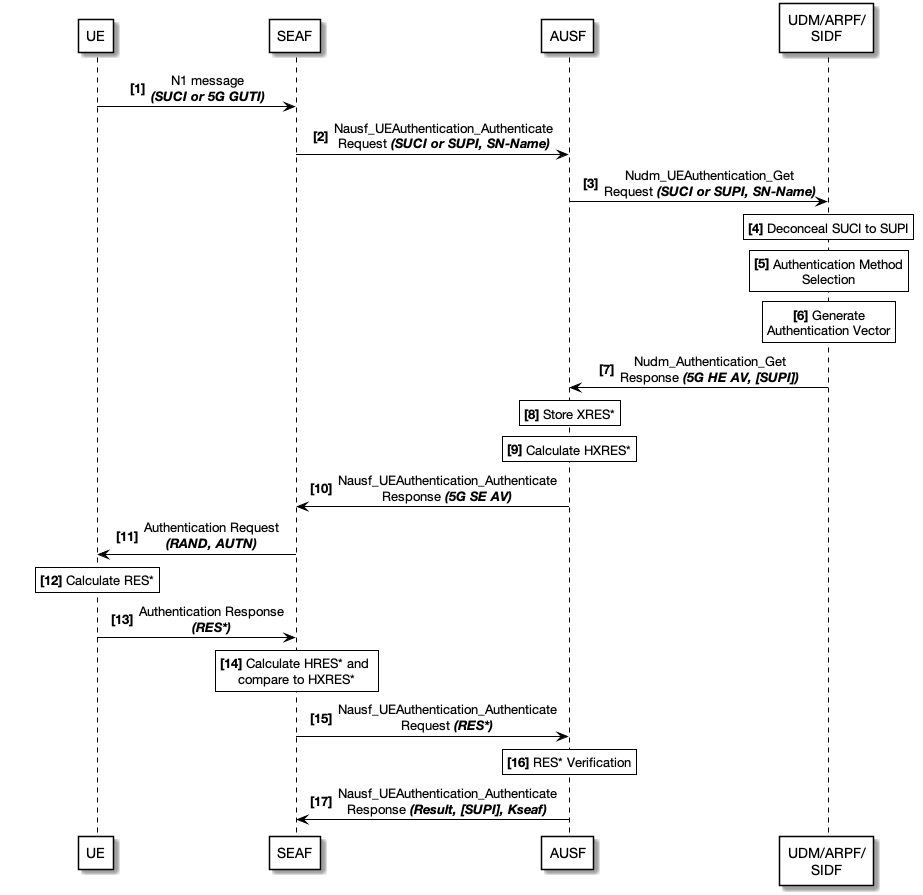
\includegraphics[width=\textwidth]{uml/protocol_v1.png}
  \caption{Das 5G-AKA Protokoll}
  \label{fig:protocol_v1}
\end{figure}

Die einzelnen Nachrichten lassen sich folgendermaßen beschreiben: %3GPP TS 33.501 V15.34.1 Page 40 und 44

\begin{enumerate}
%1
\item Das \gls{ue} sendet in Schritt 1 die \textit{N1 message} an die \gls{seaf} und beginnt damit die Authentifikationsprozedur.
Diese Nachricht beinhaltet entweder den \gls{suci} oder den \gls{5g-guti}.
Sie werden später von dem \gls{udm}/\gls{arpf} zur Authentifizierung des \gls{ue} verwendet.

%2
\item Nach dem Empfang der \textit{N1 message} sendet die \gls{seaf} in Schritt 2 den \textit{Nausf\_UEAuthentication\_ Authenticate Request} an die \gls{ausf}.
Falls in der \textit{N1 message} der \gls{5g-guti} enthalten ist und es sich um eine Re-Authentifizierung handelt, dann soll der \gls{supi} an die \gls{ausf} gesendet werden, ansonsten wird der \gls{suci} weitergeleitet.
Zusätzlich wird noch der \gls{sn-name} mitgesendet.
Dies ist nötig, da das \gls{udm} den \gls{sn-name} für die Generierung des \gls{5g-he-av} benötigt.

%3
\item Nach dem Empfang des \textit{Nausf\_UEAuthentication\_Authenticate Request}s prüft die \gls{ausf}, ob die \gls{seaf} berechtigt ist, den gesendeten \gls{sn-name} zu verwenden.
Falls dieser Test erfolgreich war, sendet die \gls{ausf} den \textit{Nudm\_UEAuthentication\_Get Request} an das \gls{udm}.
Er enthält den \gls{suci} oder \gls{supi} und den \gls{sn-name}, den die \gls{ausf} aus \textit{Schritt 2} erhalten hat.
Falls der Test nicht erfolgreich war, antwortet die \gls{ausf} mit der \textit{Nausf\_UEAuthentication\_Authenticate Response}, die den Text \textit{serving network not authorized} enthält.

%4
\item Falls die \gls{ausf} in \textit{Schritt 3} den \gls{suci} an das \gls{udm} gesendet hat, wird in diesem Schritt aus dem \gls{suci} der \gls{supi} abgeleitet.
Hierfür wird die \gls{sidf} verwendet.

%5
\item In diesem Schritt wird die Authentifikationsmethode ausgewählt.
Das \gls{udm} kann zwischen dem EAP-AKA' und dem 5G-AKA Protokoll wählen.
Da in dieser Ausarbeitung nur auf das 5G-AKA-Protokoll eingegangen wird, wird angenommen, dass hier immer das 5G-AKA-Protokoll als Authentifikationsmethode gewählt wird.

%6
\item Nun wird der \gls{5g-he-av} generiert.
Hierfür wird der \gls{sn-name} und der \gls{supi} benötigt, den das \gls{udm} in \textit{Schritt 3} erhalten oder in \textit{Schritt 4} erzeugt hat.
Für die Generierung soll das \textit{separation bit} des \gls{amf} auf ''1'' gesetzt werden.

%7
\item Jetzt sendet das \gls{udm} die \textit{Nudm\_Authentication\_Get Response} an die \gls{ausf}.
Sie beinhaltet den \gls{5g-he-av}, der in \textit{Schritt 6} generiert wurde, und den Hinweis, dass der \gls{5g-he-av} für das 5G-AKA-Protokoll bestimmt ist.
Falls das \gls{udm} in \textit{Schritt 3} den \gls{suci} erhalten und in \textit{Schritt 4} den \gls{supi} erzeugt hat, dann wird der \gls{supi} in der \textit{Nudm\_Authentication\_Get Response} mitgeschickt.

%8
\item In Schritt 8 wird die \gls{xres*}, die in dem \gls{5g-he-av} aus \textit{Schritt 7} enthalten ist, und der \gls{suci} oder \gls{supi} zwischengespeichert, da sie in \textit{Schritt 16} für die Verifikation von \gls{res*} benötigt werden.
Des Weiteren wird auch der \gls{k-ausf}, welcher auch in dem \gls{5g-he-av} enthalten ist, zwischengespeichert.

%9
\item Als nächstes wird aus der \gls{xres*} die \gls{hxres*} gerechnet.
Des Weiteren wird der \gls{5g-se-av} für \textit{Schritt 10} aus dem \gls{5g-he-av} berechnet.
Dafür wird die \gls{xres*} durch die \gls{hxres*} ersetzt und der \gls{k-ausf} entfernt.

%10
\item Nachdem der \gls{5g-se-av} in \textit{Schritt 9} erzeugt wurde wird er in Schritt 10 mit der \textit{Nausf\_UEAuthentication\_Authenticate Response} an die \gls{seaf} gesendet.
Erhält die \gls{seaf} diese Nachricht nicht, so soll mit \textit{Schritt 2'} von \cref{fig:protocol_res*_verification_failure_v1} fortgefahren werden.

%11
\item Nach dem Erhalten der \textit{Nausf\_UEAuthentication\_Authenticate Response} wird die \gls{seaf} in Schritt 11 den \textit{Authentication Request}  an das \gls{ue} schicken.
Er beinhaltet die \gls{rand} und das \gls{autn} den die \gls{seaf} in \textit{Schritt 10} erhalten hat.
Zusätzlich wird noch der \gls{ng-ksi} und die \gls{abba}, die nach einer erfolgreichen Authentifizierung benötigt werden, mitgesendet.
Des Weiteren wird die \gls{hxres*}, die in dem \gls{5g-se-av} enthalten ist, bei der \gls{seaf} zwischengespeichert, da sie noch für \textit{Schritt 14} benötigt wird.

%12
\item Nachdem das \gls{ue} den \textit{Authentication Request} von der \gls{seaf} erhalten hat, wird in Schritt 12 überprüft ob der \gls{autn} angenommen werden kann.
Ist dies der Fall, dann wird aus der \gls{rand} und dem \gls{autn} die \gls{res*} für die \textit{Authentication Response} berechnet.
Hierfür wird das \textit{separation bit} des \gls{amf} auf ''1'' gesetzt.
Es wird auch der \gls{xmac} berechnet und mit dem \gls{mac}, der in dem \gls{autn} enthalten ist, verglichen.
Stimmen \gls{xmac} und \gls{mac} überein, so wird die Authentifizierung fortgesetzt.
Stimmen sie nicht überein oder kann der \gls{autn} nicht angenommen werden, so wird die Authentifizierung als fehlgeschlagen angesehen und es wird die Prozedur aus \cref{fig:protocol_mac_failure_v1} ausgeführt.

%13
\item In Schritt 13 wird die \gls{res*}, die in \textit{Schritt 12} berechnet wurde, in der \textit{Authentication Response} vom \gls{ue} an die \gls{seaf} gesendet.

%14
\item Nachdem die \gls{seaf} die \textit{Authentication Response} vom \gls{ue} erhalten hat, berechnet sie aus der \gls{res*} die \gls{hres*} und vergleicht sie mit der \gls{hxres*}, die sie in \textit{Schritt 11} zwischengespeichert hat.
Stimmen sie überein so wird die Authentifizierung von der \gls{seaf} als erfolgreich angesehen und es geht weiter mit \textit{Schritt 15}.
Stimmen sie nicht überein, so wird die Authentifizierung von der \gls{seaf} als fehlgeschlagen angesehen und es wird die Prozedur aus dem Abschnitt \textit{HRES* failure in \gls{seaf}} in \cref{fig:protocol_res*_verification_failure_v1} ausgeführt.
Wird keine Antwort vom \gls{ue} erhalten, so wird die Authentifizierung von der \gls{seaf} als fehlgeschlagen angesehen und die \gls{ausf} wird über den Fehlschlag informiert.
Wann dieser Zeitpunkt erreicht ist, ist nicht spezifiziert.

%15
\item In Schritt 15 sendet die \gls{seaf} den \textit{Nausf\_UEAuthentication\_Authenticate Request} an die \gls{ausf}.
Er beinhaltet die \gls{res*} den die \gls{seaf} in der \textit{Authentication Response} vom \gls{ue} erhalten hat.

%16
\item Nachdem die \gls{ausf} den \textit{Nausf\_UEAuthentication\_Authenticate Request} erhalten hat vergleicht sie die \gls{res*} mit der \gls{xres*}, die sie in \textit{Schritt 8} zwischengespeichert hat.
Stimmen sie überein so wird die Authentifizierung von der \gls{ausf} als erfolgreich angesehen und es geht weiter mit \textit{Schritt 17}.
Stimmen sie nicht überein, so wird die Authentifizierung von der \gls{ausf} als fehlgeschlagen angesehen und es wird die Prozedur aus dem Abschnitt \textit{RES* failure in \gls{seaf}} in \cref{fig:protocol_res*_verification_failure_v1} ausgeführt.
Außerdem kann auch überprüft werden, ob der Authentication Vector abgelaufen ist.
Dies ist aber nicht zwingend vorgeschrieben.
Die \gls{ausf} informiert das \gls{udm} über das Ergebnis (\textit{Result}) des Vergleichs.

%17
\item In Schritt 17 sendet die \gls{ausf} die \textit{Nausf\_UEAuthentication\_Authenticate Response} an die \gls{seaf}.
Sie beinhaltet das Ergebnis des Vergleichs von \gls{res*} und \gls{xres*} aus \textit{Schritt 16}.
Stimmen \gls{res*} und \gls{xres*} überein, wird auch der \textit{Anchor Key} \gls{k-seaf} mitgesendet.
Wenn die \gls{ausf} in \textit{Schritt 7} den \gls{supi} erhalten hat, dann wird im Falle des erfolgreichen Vergleichs von \gls{res*} und \gls{xres*} der \gls{supi} nun auch an die \gls{seaf} weitergeleitet.
\end{enumerate}


\subsection{Wichtige Definitionen}
\glsunset{5g-guti}
\glsunset{5g-he-av}
\glsunset{5g-se-av}
\glsunset{abba}
\glsunset{ak}
\glsunset{amf}
\glsunset{autn}
\glsunset{auts}
\glsunset{ck}
\glsunset{f12345}
\glsunset{hres*}
\glsunset{hxres*}
\glsunset{ik}
\glsunset{imsi}
\glsunset{k}
\glsunset{k-ausf}
\glsunset{k-seaf}
\glsunset{kdf}
\glsunset{mac}
\glsunset{mcc}
\glsunset{mnc}
\glsunset{ng-ksi}
\glsunset{rand}
\glsunset{res}
\glsunset{res*}
\glsunset{sidf}
\glsunset{sn-name}
\glsunset{sqn}
\glsunset{suci}
\glsunset{supi}
\glsunset{supi-type}
\glsunset{xmac}
\glsunset{xres}
\glsunset{xres*}

%5G GUTI
\glsreset{5g-guti}
\subsubsection{\gls{5g-guti}}
Der \gls{5g-guti} ist ein Bitfeld das vom \glsunset{amf}\gls{amf} erstellt wird.
Er kann, wie auch der \gls{suci}, für die Initiierung der Authentifizierung verwendet werden.
Er besteht aus zwei Teilen mit denen man das \gls{amf} und das \gls{ue} eindeutig identifizieren kann. %3GPP TS 23.003 V15.7.0 Page 35
Diese Teile sind der \gls{guami} und der \gls{5g-tmsi}.
\begin{equation*}
\gls{5g-guti} = \gls{guami} || \gls{5g-tmsi}
\end{equation*}
\begin{equation*}
\gls{guami} = \gls{mcc} || \gls{mnc} || AMF Identifier
\end{equation*}
\begin{equation*}
AMF Identifier = AMF Region Id || AMF Set Id || AMF Pointer
\end{equation*}
Der \gls{5g-tmsi} hat eine Länge von 32 Bits, die AMF Region Id hat eine Länge von 8 Bits, die AMF Set Id hat eine Länge von 10 Bits und der AMF Pointer hat eine Länge von 6 Bits. %3GPP TS 23.003 V15.7.0 Page 36

%5G HE AV
\glsreset{5g-he-av}
\subsubsection{\gls{5g-he-av}}
Der \gls{5g-he-av} ist eine Sammlung von Zahlen und Bitfeldern, die für die Authentifizierung benötigt werden.
Er wird von dem \gls{udm} erstellt und an die \gls{ausf} geschickt.

Er beinhaltet \gls{rand}, \gls{autn}, \gls{xres*} und \gls{k-ausf}. %3GPP TS 33.501 V15.34.1 Page 44

%5G SE AV
\glsreset{5g-se-av}
\subsubsection{\gls{5g-se-av}}
Der \gls{5g-se-av} ist auch eine Sammlung von Zahlen und Bitfeldern, die für die Authentifizierung benötigt werden.
Er wird von der \gls{ausf} erstellt und an die \gls{seaf} geschickt.

Er beinhaltet \gls{rand}, \gls{autn} und \gls{hxres*}. %3GPP TS 33.501 V15.34.1 Page 44

%AUTN
\glsreset{autn}
\subsubsection{\gls{autn}}
Der \gls{autn} ist ein Bitfeld und besteht aus den drei Komponenten \gls{sqn}, \gls{ak}, \gls{amf} und \gls{mac}. 
Er ist wie folgt aufgebaut: %3GPP TS 33.102 V15.1.0 Page 25
\begin{equation*}
\gls{autn} = (\gls{sqn} \oplus \gls{ak}) || \gls{amf} || \gls{mac}
\end{equation*}
\begin{itemize}
\item Das \gls{amf} wird benötigt, um \gls{mac} zu berechnen und um spezifische Anpassungen vorzunehmen.
\item Der \gls{mac} wird benötigt, um ihn mit dem \gls{xmac} zu vergleichen.
\item Die \gls{sqn}$ \oplus $\gls{ak} soll die \gls{sqn} übermitteln.
Sie wird mit dem \gls{ak} verschlüsselt um die Identität und Position der Benutzers nicht preiszugeben.
Ist \gls{ak} = 0, dann kann davon ausgegangen werden dass die \gls{sqn} alleine weder Identität noch Position des Benutzers preisgibt.
\end{itemize}

%HRES*
\glsreset{hres*}
\subsubsection{\gls{hres*}}
\gls{hres*} ist der Hash von \gls{res*} und wird von der \gls{seaf} benötigt, um ihn mit dem \gls{hxres*} zu vergleichen.
Er wird von der \gls{seaf} mit Hilfe des SHA-256-Algorithmus berechnet. %3GPP TS 33.501 V15.34.1 Page 155
Eingabe des SHA-256-Algorithmus ist die Konkatenation von \gls{rand} und \gls{res*} (\gls{rand} || \gls{res*}).

\gls{hres*} setzt sich aus den 128 \textit{least significant} Bits von der Ausgabe des SHA-256 zusammen.

%HXRES*
\glsreset{hxres*}
\subsubsection{\gls{hxres*}}
\gls{hxres*} ist der Hash von \gls{xres*} und wird von der \gls{seaf} benötigt, um ihn mit dem \gls{hres*} zu vergleichen.
Er wird von der \gls{ausf} mit Hilfe des SHA-256-Algorithmus berechnet. %3GPP TS 33.501 V15.34.1 Page 155
Eingabe des SHA-256-Algorithmus ist die Konkatenation von \gls{rand} und \gls{xres*} (\gls{rand} || \gls{xres*}).

\gls{hxres*} setzt sich aus den 128 \textit{least significant} Bits von der Ausgabe des SHA-256 zusammen.

%K
\glsreset{k}
\subsubsection{\gls{k}}
Der Schlüssel \gls{k} hat Länge von 128 oder 256 Bits und wird für die Generierung von \gls{ak}, \gls{ck}, \gls{ik} \gls{res} bzw. \gls{xres} und \gls{mac} bzw. \gls{xmac} benötigt. %3GPP TS 33.102 V15.1.0 Page 32
Die tatsächliche Länge ist nicht spezifiziert und wird möglicherweise von Provider festgelegt. %3GPP TS 33.102 V15.1.0 Page 32

\gls{k} soll auf dem \gls{udm}/\gls{arpf} und in einer manipulationssicheren Hardwarekomponente auf dem \gls{ue} gespeichert werden.  %3GPP TS 33.501 V15.34.1 Page 29

%K_SEAF
\glsreset{k-seaf}
\subsubsection{\gls{k-seaf}}
Der \gls{k-seaf}, auch \textit{Anchor Key} genannt, ist der Schlüssel auf den sich alle Entitäten bei erfolgreicher Authentifizierung einigen. %3GPP TS 33.501 V15.34.1 Page 37
Er wird von der \gls{ausf} und dem \gls{ue} berechnet und lässt sich mit Hilfe der \gls{kdf} berechnen.
Dabei sind folgende Werte Eingabeparameter der \gls{kdf}: %3GPP TS 33.501 V15.34.1 Page 155
\begin{itemize}
\item KEY = \gls{k-ausf}
\item Fc = 0x6C
\item P0 = \gls{sn-name}
\end{itemize}
Die Ausgabe der \gls{kdf} ist der \gls{k-seaf}.

\glsreset{rand}
\subsubsection{\gls{rand}}
Der \gls{rand} ist eine 128 Bit lange zufällige Zahl. %3GPP TS 33.102 V15.1.0 Page 32
Sie wird für die Generierung von \gls{ak}, \gls{ck}, \gls{ik} \gls{res} bzw. \gls{xres} und \gls{mac} bzw. \gls{xmac} benötigt. 
Der \gls{rand} soll eine unvorhersehbare Zahl sein, wie genau sie generiert wird ist jedoch nicht beschrieben. %3GPP TS 33.102 V15.1.0 Page 25

Sie wird vom \gls{udm}/\gls{arpf} erzeugt und an das \gls{ue} weitergeleitet. Diese Entitäten generieren auch die oben genannten Schlüssel \gls{ak}, \gls{ck}, \gls{ik}, usw.

%RES*
\glsreset{res*}
\subsubsection{\gls{res*}}
Die \gls{res*} ist eine Bitfolge und lässt sich, wie auch \gls{xres*}, mit Hilfe der \gls{kdf} berechnen.
Dabei sind folgende Werte Eingabeparameter der \gls{kdf}: %3GPP TS 33.501 V15.34.1 Page 155
\begin{itemize}
\item KEY = Konkatenation von \gls{ck} und \gls{ik} (\gls{ck} || \gls{ik})
\item Fc = 0x6B
\item P0 = \gls{sn-name}
\item P1 = \gls{rand}
\item P2 = \gls{res}
\end{itemize}

\gls{res*} setzt sich aus den 128 \textit{least significant} Bits von der Ausgabe der \gls{kdf} zusammen.
\gls{res*} wird für die Berechnung von \gls{hres*} benötigt.
Es wird vom \gls{ue} berechnet.

%SN-Name
\glsreset{sn-name}
\subsubsection{\gls{sn-name}}
Der \gls{sn-name} wird für die Berechnung von \gls{res*} bzw. \gls{xres*}, \gls{k-ausf} und \gls{k-seaf} benötigt.
Er hat zwei Zwecke: %3GPP TS 33.501 V15.34.1 Page 39
\begin{itemize}
\item Er bindet den \gls{k-seaf}, auch  \textit{Anchor Key}  genannt, an die \gls{seaf}, auch \textit{Serving Network} genannt, indem es die \gls{sn-id} beinhaltet.
\item Er stellt sicher, dass der \textit{Anchor Key} nur für die Authentifizierung in 5G-Netzwerken verwendbar ist, indem es den Service Code ''5G'' beinhaltet.
\end{itemize}
Der \gls{sn-name} ist wie folgt aufgebaut: %3GPP TS 33.501 V15.34.1 Page 39

Er beginnt mit dem Service code ''5G'' gefolgt von dem Trennzeichen '':'' und der \gls{sn-id}.
Die \gls{sn-id} ist für jedes \textit{Serving Network} eindeutig.
\begin{equation*}
\gls{sn-name} = ''5G'' || '':'' || \gls{sn-id}
\end{equation*}
\begin{equation*}
\gls{sn-id} = \gls{mcc} || \gls{mnc}
\end{equation*}

%SUCI
\glsreset{suci}
\subsubsection{\gls{suci}}
Der \gls{suci} ist die verschlüsselte Version des \gls{supi} und wird für die Identifizierung des \gls{ue} benötigt..
Er lässt sich mit der \gls{sidf} in den \gls{supi} umwandeln.

Er ist wie folgt aufgebaut: %3GPP TS 23.003 V15.7.0 Page 27

\gls{suci} = \gls{supi-type} || Home Network Identifier || Routing Indicator || Protection Scheme Id || Home Network Public Key Id || Scheme Output

\begin{itemize}
\item Der Home Network Identifier ist von dem \gls{supi-type} abhängig.
\begin{itemize}
\item Wenn der \gls{supi-type} den \gls{imsi} angibt, dann entspricht der Home Network Identifier dem \gls{mcc} gefolgt von dem \gls{mnc} (Home Network Identifier = \gls{mcc} || \gls{mnc}). 
\item Wenn der \gls{supi-type} den Network Specific Identifier angibt, dann entspricht der Home Network Identifier einer ähnlichen Form des Network Access Identifiers, wie er beim \gls{supi} verwendet wird. (Home Network Identifier = username@realm)
Er ist genauer im Dokument IETF RFC 7542 spezifiziert. %IETF RFC 7542 Page 10 fort folgend
\end{itemize}
\item Der Routing Indicator besteht aus 1 bis zu 4 Zeichen. %3GPP TS 23.003 V15.7.0 Page 28
Er erlaubt es der \gls{seaf} zusammen mit dem Home Network Identifier eine Verbindung mit der korrekten \gls{ausf} aufzubauen.
Falls kein Routing Indicator konfiguriert ist soll er auf 0 gesetzt werden.
\item Der Protection Scheme Identifier kann Werte von 0 bis 15 annehmen.
Die genaue Definition der einzelnen Algorithmen ist im Annex C des 3GPP TS 33.501 V15.34.1 zu finden. %3GPP TS 33.501 V15.34.1 Page 168
\begin{itemize}
\item Der Wert 0 bedeutet, dass das Null Scheme verwendet wird.
\item Der Wert 1 bedeutet, dass das Profile A verwendet wird.
\item Der Wert 2 bedeutet, dass das Profile B verwendet wird.
\item Die Werte 3 bis 11 sind für zukünftige Spezifikationen reserviert.
\item Die Werte 12 bis 15 sind für spezifische Algorithmen reserviert.
\end{itemize}
\item Der Home Network Public Key Identifier kann Werte von 0 bis 255 annehmen.
Er wird genutzt den Public Key zu identifizieren, der für die Verschlüsselung des \gls{supi} verwendet wird.
\item Der Scheme Output ist die Ausgabe des Verschlüsselungs-Algorithmus.
Die genaue Definition des Scheme Outputs ist im Annex C des 3GPP TS 33.501 V15.34.1 zu finden. %3GPP TS 33.501 V15.34.1 Page 168
\end{itemize}

%SUPI
\glsreset{supi}
\subsubsection{\gls{supi}}
Der \gls{supi} wird für die Identifizierung des \gls{ue} benötigt.
Er ist für jeden Nutzer global eindeutig. 
Er ist wie folgt aufgebaut: %3GPP TS 23.003 V15.7.0 Page 27

\gls{supi} = \gls{supi-type} || Home Network Identifier

Der Identifier ist von dem \gls{supi-type} abhängig und kann folgende Werte annehmen:

\begin{itemize}
\item Wenn der \gls{supi-type} den \gls{imsi} angibt, dann entspricht der Home Network Identifier dem \gls{imsi}. (Home Network Identifier = \gls{imsi})
\item Wenn der \gls{supi-type} den Network Specific Identifier angibt, dann entspricht der Home Network Identifier dem Network Access Identifier. (Home Network Identifier = Network Access Identifier)
Der Network Access Identifier hat die Form $ username@realm $. 
Er ist genauer im Dokument IETF RFC 7542 spezifiziert. %IETF RFC 7542 Page 10 fort folgend
\end{itemize}

%XRES*
\glsreset{xres*}
\subsubsection{\gls{xres*}}
Die \gls{xres*} ist eine Bitfolge und lässt sich, wie auch \gls{res*}, mit Hilfe der \gls{kdf} berechnen.
Dabei sind folgende Werte Eingabeparameter der \gls{kdf}: %3GPP TS 33.501 V15.34.1 Page 155
\begin{itemize}
\item KEY = Konkatenation von \gls{ck} und \gls{ik} (\gls{ck} || \gls{ik})
\item Fc = 0x6B
\item P0 = \gls{sn-name}
\item P1 = \gls{rand}
\item P2 = \gls{xres}
\end{itemize}

\gls{xres*} setzt sich aus den 128 \textit{least significant} Bits von der Ausgabe der \gls{kdf} zusammen.
\gls{xres*} wird für die Berechnung von \gls{hxres*} benötigt.
Es wird von der \gls{arpf} berechnet.


\subsection{Weitere Begriffe}

%ABBA
\glsreset{abba}
\subsubsection{\gls{abba}}
Der \gls{abba} Parameter soll einen \textit{Anti-bidding down}-Schutz für Sicherheitsfeatures gewährleisten, die es verhindern sollen, dass ältere Sicherheitsfeatures verwendet werden obwohl alle Parteien neuere Sicherheitsfeatures unterstützen. %3GPP TS 33.501 V15.34.1 Page 22
Des Weiteren soll damit angegeben werden welche Sicherheitsfeatures in diesem Netzwerk aktiv sind.

Der \gls{abba} Parameter wird von der \gls{seaf} an das \gls{ue} gesendet und hat eine variable Länge.
Zurzeit kann der \gls{abba} Parameter nur den Wert 0x0000 annehmen. Dieser Wert steht für die bisher definierten Sicherheitsfeatures. %3GPP TS 33.501 V15.34.1 Page 156

%AK
\glsreset{ak}
\subsubsection{\gls{ak}}
Der \gls{ak} ist ein Schlüssel mit einer Länge von 48 Bits.
Er wird zum Verschlüsseln der \gls{sqn} verwendet. %3GPP TS 33.102 V15.1.0 Page 32
Lässt die \gls{sqn} keine Rückschlüsse auf die Identität oder Position der Nutzers zu, so kann der \gls{ak} auch auf 0 gesetzt werden. %3GPP TS 33.102 V15.1.0 Page 25

Der \gls{ak} wird mit der \textit{Key generating function} f5 berechnet und bekommt \gls{rand} und \gls{k} als Eingabe. %3GPP TS 33.102 V15.1.0 Page 26

%AMF
\glsreset{amf}
\subsubsection{\gls{amf}}
Das \gls{amf} ist ein 16 Bit langes Bitfeld. %3GPP TS 33.102 V15.1.0 Page 32
Es wird für die Berechnung von Tokens und anderen Bitfeldern benötigt.
Die 16 Bits des \gls{amf} sind von 0 bis 15 durchnummeriert. %3GPP TS 33.102 V15.1.0 Page 79
0 steht hier für das \textit{most significant bit} und 15 steht für das \textit{least significant bit}.

\begin{itemize}
\item Bit 0, auch \textit{separation bit} genannt, wird für das \gls{eps} verwendet und wird bei der Verwendung des \gls{amf} meist explizit angegeben. \\
\item Bits 1 bis 7 sind für eine zukünftige Spezifikation reserviert und sollen auf 0 gesetzt werden. \\
\item Bits 8 bis 15 können für proprietäre Zwecke verwendet werden, sind aber nicht explizit festgelegt. 
Sie können verwendet werden um spezifische Anpassungen festzulegen.
Zum Beispiel könnten mehrere Authentifikations-Algorithmen unterstützt werden, indem die Bits 8 bis 15 den Algorithmus festlegen oder es könnten die Verifikationsparameter der \gls{sqn} durch die Bits bestimmt werden. %3GPP TS 33.102 V15.1.0 Page 77
\end{itemize}

%AUTS
\glsreset{auts}
\subsubsection{\gls{auts}}
Der \gls{auts} Parameter wird für die Re-Synchronisations Prozedur aus \textit{Schritt 3*} von \cref{fig:protocol_mac_failure_v1} benötigt.
Die \gls{seaf} erhält den \gls{auts} Parameter von dem \gls{ue} nach einer beim \gls{ue} fehlgeschlagenen Authentifizierung.
\begin{equation*}
\gls{auts} = Conc(\gls{sqn}) || MACS
\end{equation*}
\begin{equation*}
Conc(\gls{sqn}) = \gls{sqn} \oplus f5*(RAND)
\end{equation*}
\begin{equation*}
MACS = f1*(\gls{sqn} || \gls{rand} || \gls{amf})
\end{equation*}
Die Funktionen f1* und f5* sind, wie auch die \textit{Message authentication and Key generating functions} vom \gls{k} abhängig, dürfen aber keine Schlüsse über die Funktionen \gls{f12345} zulassen.

%CK
\glsreset{ck}
\subsubsection{\gls{ck}}
Der \gls{ck} ist ein 128 Bit langer Schlüssel. %3GPP TS 33.102 V15.1.0 Page 32
Er wird, zusammen mit dem \gls{ik}, benötigt um den \gls{k-ausf} zu berechnen.

Der \gls{ck} wird von der \textit{Key generating function} f3 berechnet.
Diese Funktion bekommt \gls{rand} und \gls{k} als Eingabe. %3GPP TS 33.102 V15.1.0 Page 26

%f1, f2, f3, f4, f5
\glsreset{f12345}
\subsubsection{\gls{f12345}}
Mit diesen Funktionen werden \gls{ak}, \gls{ck}, \gls{ik} \gls{res} bzw. \gls{xres} und \gls{mac} bzw. \gls{xmac} berechnet. %3GPP TS 33.102 V15.1.0 Page 26
\begin{itemize}
\item Bei f1 handelt es sich um eine \textit{Message authentication function}.
Sie berechnet den \gls{mac} bzw. \gls{xmac} und bekommt \gls{k} und die Konkatenation von \gls{sqn}, \gls{rand} und \gls{amf} (\gls{sqn} || \gls{rand} || \gls{amf}) als Eingabe. \\
\item Bei f2 handelt es sich um eine, möglicherweise verkürzte, \textit{Message authentication function}.
Sie berechnet die \gls{res} bzw. \gls{xres} und bekommt \gls{k} und \gls{rand} als Eingabe.
\item Bei f3, f4 und f5 handelt es sich um \textit{Key generating function}s.
f3 berechnet \gls{ck}, f4 berechnet \gls{ik} und f5 berechnet \gls{ak}.
Alle drei Funktionen bekommen \gls{k} und \gls{rand} als Eingabe.
Falls \gls{sqn} keine Rückschlüsse auf die Identität oder Position des Benutzers zulässt wird f5 = 0 gesetzt.
\end{itemize}

%IK
\glsreset{ik}
\subsubsection{\gls{ik}}
Der \gls{ik} ist ein 128 Bit langer Schlüssel. %3GPP TS 33.102 V15.1.0 Page 32
Er \gls{ik} wird, zusammen mit dem \gls{ck}, benötigt um \gls{k-ausf} zu berechnen.

Er wird von der \textit{Key generating function} f4 berechnet.
Diese Funktion bekommt \gls{rand} und \gls{k} als Eingabe. %3GPP TS 33.102 V15.1.0 Page 26

%IMSI
\glsreset{imsi}
\subsubsection{\gls{imsi}}
Die \gls{imsi} ist bis zu 15 Zahlen lange Zahlenfolge und wird unter anderem für die Identifizierung des \gls{ue} benötigt.
Die \gls{imsi} darf nur aus den Dezimalzahlen 0 - 9 bestehen. %3GPP TS 23.003 V15.7.0 Page 29
Sie wird aus dem \gls{mcc}, dem \gls{mnc} und der \gls{msin} aufgebaut. %3GPP TS 23.003 V15.7.0 Page 26
\begin{equation*}
\gls{imsi} = \gls{mcc} || \gls{mnc} || \gls{msin}
\end{equation*}
Die \gls{msin} ist bis zu 9 Zahlen lang und identifiziert den Benutzer eindeutig. %3GPP TS 23.003 V15.7.0 Page 26

%K_AUSF
\glsreset{k-ausf}
\subsubsection{\gls{k-ausf}}
Der \gls{k-ausf} wird für die Berechnung des \gls{k-seaf} benötigt.
Er lässt sich mit Hilfe der \gls{kdf} berechnen.
Dabei sind folgende Werte Eingabeparameter der \gls{kdf}: %3GPP TS 33.501 V15.34.1 Page 154
\begin{itemize}
\item KEY = Konkatenation von \gls{ck} und \gls{ik} (\gls{ck} || \gls{ik})
\item Fc = 0x6A
\item P0 = \gls{sn-name}
\item P1 = Konkatenation von \gls{sqn} und \gls{ak} (\gls{sqn} || \gls{ak}).
\end{itemize}
Die Ausgabe der \gls{kdf} ist der \gls{k-ausf}.

\gls{k-ausf} wird von der \gls{arpf} und dem \gls{ue} berechnet und wird für die Berechnung von \gls{k-seaf} benötigt.

%KDF
\glsreset{kdf}
\subsubsection{\gls{kdf}}
Die \gls{kdf} wird für die Berechnung von \gls{k-ausf}, \gls{k-seaf} und \gls{res*} bzw. \gls{xres*} benötigt.

Die Eingabeparameter der \gls{kdf} sind KEY, Fc, P0, $ \dots $, Pn und optional auch L0, $ \dots $, Ln.

Um den Schlüssel zu berechnen muss zuerst der Wert S berechnet werden. %3GPP TS 33.220 V15.4.0 Page 46
Er l\"asst sich folgendermaßen zusammensetzen: 
\begin{equation*}
S = Fc || P0 || L0 || P1 || L1 || \dots || Pn || Ln 
\end{equation*}
Die Länge von allen P1, $ \dots $, Pn ist durch 8 teilbar und L1, $ \dots $, Ln sind genau 16 Bit groß und geben die Längen der Parameter P1, $ \dots $, Pn an. 
Das heißt, dass Li die Anzahl der Bytes, die mindestens benötigt werden um Pi zu speichern, binär in 16 Bits kodiert. \\
Zum Beispiel: Ist P0 16 Bit und P1 24 Bit lang, dann hat L0 den Wert 0x02 und L1 den Wert 0x03.

Die Ausgabe der \gls{kdf} ist das Ergebnis folgender Rechnung: \\
Ausgabe = HMAC-SHA-256(KEY, S) \\

%MAC
\glsreset{mac}
\subsubsection{\gls{mac}}
Der \gls{mac} hat eine Länge von 64 Bits und wird vom \gls{ue} benötigt um ihn mit dem \gls{xmac} zu vergleichen.
Er wird, wie auch der \gls{xmac}, mit der \textit{Message authentication function} f1 berechnet. %3GPP TS 33.102 V15.1.0 Page 32
Die Funktion f1 ist von \gls{k} abhängig und bekommt als Eingabe die Konkatenation von \gls{sqn}, \gls{rand} und \gls{amf} (\gls{sqn} || \gls{rand} || \gls{amf}). %3GPP TS 33.102 V15.1.0 Page 26
Der \gls{mac} wird von der \gls{udm}/\gls{arpf} berechnet.

%MCC
\glsreset{mcc}
\subsubsection{\gls{mcc}}
Der \gls{mcc} ist drei Zeichen lang und ist Teil der \gls{imsi} und des \gls{sn-name}. %3GPP TS 23.003 V15.7.0 Page 26
Er identifiziert das Land in dem sich der Provider befindet. 

%MNC
\glsreset{mnc}
\subsubsection{\gls{mnc}}
Der \gls{mnc} ist zwei oder drei Zeichen lang, wie auch der \gls{mcc}, Teil der \gls{imsi} und des \gls{sn-name}. %3GPP TS 23.003 V15.7.0 Page 26
Die genaue Länge ist vom \gls{mcc} abhängig und somit von Land zu Land unterschiedlich.
Der \gls{mnc} und der \gls{mcc} zusammen identifizieren den Provider.

%ng-KSI
\glsreset{ng-ksi}
\subsubsection{\gls{ng-ksi}}
Der \gls{ng-ksi} identifiziert den K\textsubscript{AMF} eindeutig. %3GPP TS 33.501 V15.34.1 Page 54
Er wird von der \gls{seaf} an das \gls{ue} geschickt und wird nach einer erfolgreichen Authentifizierung benötigt um den K\textsubscript{AMF} zu identifizieren.

%RES
\glsreset{res}
\subsubsection{\gls{res}}
Die \gls{res} ist eine Bitfolge mit einer variablen Länge von bis zu 416 Bytes. %3GPP TS 33.102 V15.1.0 Page 32
Sie wird von dem \gls{ue} mit der \textit{Message authentication function} f2 berechnet.
Die Funktion bekommt \gls{k} und \gls{rand} als Eingabe. %3GPP TS 33.102 V15.1.0 Page 26

Die \gls{res} wird von der \gls{ausf} mit der \gls{xres} verglichen.
Stimmen sie nicht überein so bricht die \gls{ausf} die Authentifizierung ab. %3GPP TS 33.501 V15.34.1 Page 45

%SQN
\glsreset{sqn}
\subsubsection{\gls{sqn}}
\gls{sqn} ist eine Zahl mit einer Länge von 48 Bits. %3GPP TS 33.102 V15.1.0 Page 32
Aus ihr wird der \gls{mac} bwz. \gls{xmac} erzeugt. %3GPP TS 33.102 V15.1.0 Page 25

Für die Generierung der \gls{sqn} muss das \gls{udm}/\gls{arpf} folgende Bedingungen erfüllen:\\%3GPP TS 33.102 V15.1.0 Page 25
\begin{enumerate}
\item Der Erzeugungsmechanismus der \gls{sqn} soll eine Re-Synchronisations Prozedur beinhalten.
Die Re-Synchronisations Prozedur ist eine Prozedur die ausgeführt werden kann, wenn der \gls{autn} vom \gls{ue} in \textit{Schritt 1*} von \cref{fig:protocol_mac_failure_v1} nicht angenommen werden kann (\textit{Synchronization failure}).
\item Der Erzeugungsmechanismus soll gegen den Überlauf der \gls{sqn} (\textit{Wrap around Protection}) geschützt sein, da sonst eine bereits verwendete \gls{sqn} möglicherweise erneut erzeugt und verwendet werden könnte. 
\end{enumerate}

Falls die \gls{sqn} Rückschlüsse auf die Identität oder Position des Nutzers zulässt, dann soll der \gls{ak} verwendet werden um die \gls{sqn} zu verbergen.

%SUPI-Type
\glsreset{supi-type}
\subsubsection{\gls{supi-type}}
Der \gls{supi-type} wird zum Erzeugen des \gls{supi} benötigt und kann Werte von 0 bis 7 annehmen. %3GPP TS 23.003 V15.7.0 Page 27
\begin{itemize}
\item Der Wert 0 bedeutet, dass der Home Network Identifier den \gls{imsi} angibt.
\item Der Wert 1 bedeutet, dass der Home Network Identifier den Network Specific Identifier angibt.
\item Die Werte 2 bis 7 sind für zukünftige Spezifikation reserviert.
\end{itemize}

%XMAC
\glsreset{xmac}
\subsubsection{\gls{xmac}}
Der \gls{xmac} hat eine Länge von 64 Bits und wird vom \gls{ue} benötigt um ihn mit dem \gls{mac} zu vergleichen.
Er wird, wie auch der \gls{mac}, mit der Funktion f1 berechnet. %3GPP TS 33.102 V15.1.0 Page 32
Die \textit{Message authentication function} f1 bekommt als Eingabe \gls{k} und die Konkatenation von \gls{sqn}, \gls{rand} und \gls{amf} (\gls{sqn} || \gls{rand} || \gls{amf}). %3GPP TS 33.102 V15.1.0 Page 27

Der \gls{xmac} wird von dem \gls{ue} berechnet und mit dem \gls{mac} verglichen. 
Den \gls{mac} hat das \gls{ue} bereits von der \gls{seaf} erhalten.
Stimmen \gls{mac} und \gls{xmac} nicht überein, so ist die Authentifizierung fehlgeschlagen. %3GPP TS 33.102 V15.1.0 Page 27

%XRES
\glsreset{xres}
\subsubsection{\gls{xres}}
Die \gls{xres} ist eine Bitfolge mit einer variablen Länge von bis zu 416 Bytes. %3GPP TS 33.102 V15.1.0 Page 32
Sie wird, wie auch die \gls{res}, mit der \textit{Message authentication function} f2 berechnet. 
Diese Funktion bekommt \gls{k} und \gls{rand} als Eingabe. %3GPP TS 33.102 V15.1.0 Page 26

Die \gls{ausf} vergleicht \gls{res} und \gls{xres} miteinander.
Stimmen sie nicht überein, so bricht die \gls{ausf} die Authentifizierung ab. %3GPP TS 33.501 V15.34.1 Page 45


\subsection{Fehlgeschlagene Authentifikation}

\subsubsection{Fehlschlag beim Vergleich von \gls{mac} und \gls{xmac}}

\begin{figure}[H]
  \centering
  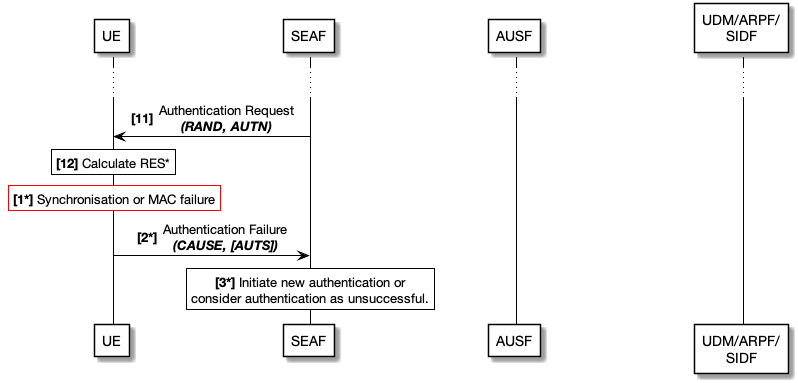
\includegraphics[width=\textwidth]{uml/protocol_mac_failure_v1.png}
  \caption{Fehlschlag beim Vergleich von \gls{mac} und \gls{xmac}}
  \label{fig:protocol_mac_failure_v1}
\end{figure}

\begin{enumerate}
%1*
\item[1*.] In Schritt 1* wird festgestellt, dass der berechnete \gls{xmac} nicht mit dem \gls{mac}, der in Schritt 11 empfangen wurde, übereinstimmt (\textit{MAC failure}) oder, dass der \gls{autn} nicht angenommen werden kann (\textit{Synchronisation failure}).

%2*
\item[2*.] In Schritt 2* sendet das \gls{ue} die \textit{Authentication Failure} an die \gls{seaf}.
Sie beinhaltet den CAUSE Wert, welcher den Grund für das Fehlschlagen beschreibt.
Handelt es sich um eine \textit{Synchronisation failure} so wird auch der \gls{auts} Parameter mitgesendet.

%3*
\item[3*.] In Schritt 3* wird entschieden ob die Authentifikation gescheitert ist oder ob eine neue Authentifikation initiiert werden soll.
eine neue Authentifikation kann nur initiiert werden wenn es sich bei dem Fehlschlag um eine \textit{Synchronisation failure} handelt.
Die genaue Beschreibung der Re-Authentifizierungsprozedur ist im Dokument TS 24.501 zu finden. %3GPP TS 24.501 V16.1.0
\end{enumerate}


\subsubsection{Fehlschlag beim Vergleich von \gls{res*} bzw. \gls{hres*} mit \gls{xres*} bzw. \gls{hxres*}}

\begin{figure}[H]
  \centering
  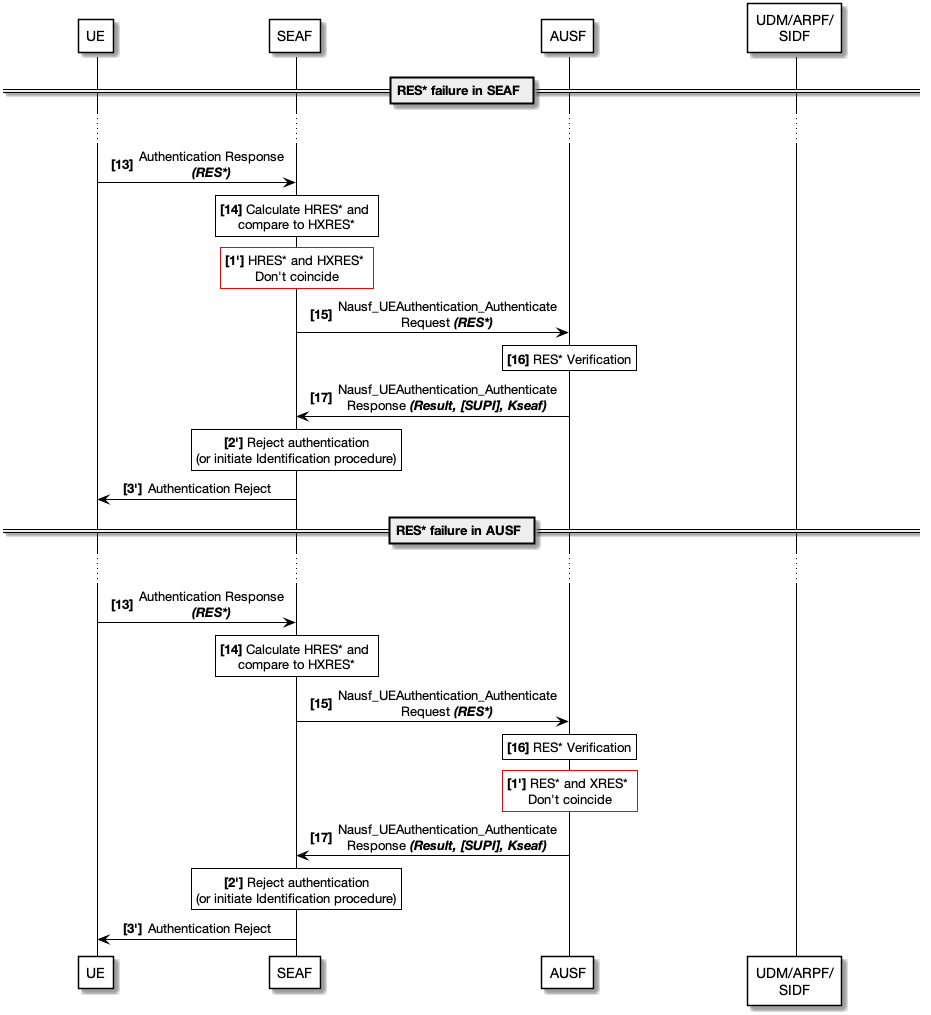
\includegraphics[width=\textwidth]{uml/protocol_res*_verification_failure_v1.png}
  \caption{Fehlschlag beim Vergleich von \gls{res*} bzw. \gls{hres*} mit \gls{xres*} bzw. \gls{hxres*}}
  \label{fig:protocol_res*_verification_failure_v1}
\end{figure}

\begin{enumerate}
%1'
\item[1'.] Im Abschnitt \textit{''HRES* failure in SEAF''} wird bei Schritt 1' festgestellt, dass \gls{hres*} und \gls{hxres*}, die in \textit{Schritt 14} verglichen wurden, nicht übereinstimmen. 
Es wird trotzdem die Nachricht aus \textit{Schritt 15} gesendet und auf die Antwort der \gls{ausf} gewartet. \\
Im Abschnitt \textit{''RES* failure in AUSF''} wird bei Schritt 1' festgestellt, dass \gls{res*} und \gls{xres*}, die in \textit{Schritt 16} verglichen wurden, nicht übereinstimmen.
Dies wird der \gls{seaf} in \textit{Schritt 17} mit dem \textit{Result} Parameter mitgeteilt.

%2'
\item[2'.] Im Schritt 2' wird die Authentifizierung als nicht erfolgreich angesehen und es wird entweder eine neue Authentifizierung initiiert oder die Authentifizierung wird abgebrochen.
Dies ist der Fall wenn der Vergleich aus dem \textit{Schritt 1'} im Abschnitt \textit{''RES* failure in AUSF''} oder im Abschnitt \textit{''HRES* failure in SEAF''} fehlschlägt.
Schlägt er in \textit{Schritt 1'} aus Abschnitt \textit{''HRES* failure in SEAF''} fehl, so wird unabhängig von dem \textit{Result} Parameter aus \textit{Schritt 17} die Authentifizierung als nicht erfolgreich angesehen.
Des Weiteren wird die Authentifizierung als nicht erfolgreich angesehen wenn die Nachricht aus \textit{Schritt 10} nicht von der \gls{seaf} erhalten wird.
Die Authentifizierung wird abgebrochen wenn die \gls{seaf} in \textit{Schritt 1} den \gls{suci} erhalten hat.
Falls die \gls{seaf} in \textit{Schritt 1} den \gls{5g-guti} erhalten hat, so soll die \textit{Identification procedure} gestartet werden, durch die die \gls{seaf} den \gls{suci} vom \gls{ue} erhalten soll.

%3'
\item[3'.] Falls in \textit{Schritt 1} die \gls{seaf} den \gls{suci} erhalten hat soll in Schritt 3' die \textit{Authentication Reject} Nachricht an das \gls{ue} gesendet werden.
\end{enumerate}













